% Author: Andrew J Young
% Compiler: XELatex


\documentclass{article}

%% Begin package imports %%%%%%%%%%%%%%%%%%%%%%%%%%%%%%%%%%%%%%%%%%%%%%%%%%%%%%%

% Language and font encodings
\usepackage[english]{babel}
% Package for angle quotes etc.
\usepackage[T1]{fontenc}
% Set page size and margins
\usepackage[a4paper,top=3cm,bottom=2cm,left=3cm,right=3cm,marginparwidth=1.75cm]{geometry}
\usepackage[utf8]{inputenc}
\usepackage{mathptmx} % TimesNewRoman-esque font
\usepackage{hyperref} % In-document referencing.
\usepackage{xeCJK} % For CJK characters.
\usepackage{wrapfig} % For wrapping text around figures.

%%%%%%%%%%%%%%%%%%%%%%%%%%%%%%%%%%%%%%%%%%%%%%%%%%%%%%%%% End package imports %%
%% Begin newcommands %%%%%%%%%%%%%%%%%%%%%%%%%%%%%%%%%%%%%%%%%%%%%%%%%%%%%%%%%%%

\newcommand{\h}[1]{$^{#1}$}
\newcommand{\s}[1]{$_{#1}$}

%%%%%%%%%%%%%%%%%%%%%%%%%%%%%%%%%%%%%%%%%%%%%%%%%%%%%%%%%%%%% End newcommands %%

\title{Iteration marks for the latin script}
\author{Andrew J. Young}

\begin{document}
\maketitle

\begin{abstract}
  Iteration marks are a feature common to many languages. Most familiarly, latin
  script languages make use of the \textit{ditto mark} to indicate a repeated
  word or phrase. While iteration marks are not uncommon to any language, they
  are often considered to be informal, or otherwise not frequently made use of
  in standardized text.

  However, this is not the case for the japanese language. The japanese writing
  system frequently and systematically uses iteration marks, including in formal
  and historic texts. This dramatically affects the writing style of japanese
  texts, and allows omission of entire phrases and syllables, as well as
  reducing stroke counts for using kanji (sinographs) in Japanese text.

  This article is a proposal for an arbitrary system of marking repeated
  characters, syllables, and words, using a slightly modified version of the
  syntax of \textit{regular expressions}. Regular expressions are a syntax for
  matching passages of text on computers, using a sophisticated and advanced
  set of symbols to mark repetition, without ambiguity.

  In particular, the following notation is proposed:
  \begin{itemize}
    \item Superscript for marking immediate repetition ($ a^3 = aaa $;
      $ hono(lu)^2 = honolulu $)
    \item Subscript for enumerating and later referencing sections of text (
      w(ork)\s{1} schm(1) = work schmork; (itsy)\s{1} b(1) = itsy bitsy)
  \end{itemize}
\end{abstract}

\section{A background to iteration}

Iteration is repetition; and repetition is a powerful tool.

Iteration has always played a powerful part in our culture and societies.
Through repetition, we can learn; we can emphasize; and we can create rules and
customs from this same repetition.

Language is no different. As an art form interwoven into human culture, language
has made full use of iteration. In English, iteration is used mostly for stress.
Nonetheless, repetition comes up all the time in our language. Just as looking
up at a \textit{blue blue sky} produces imagery of a wondrous expanse of blue,
being asked if you want soy milk at a coffee shop may be met with an irritable
«No, I want \textit{milk} milk».

Iteration can also be used to pluralize words in many languages, or even as the
default way to express the idea of being \textit{very} something. Word upon
word, iteration adds expression to languages, and is integral to how they are
used.

Because of this, and equally as humanly, these iterations have been abbreviated
over the years. A \textit{ditto} mark is the common notation in english to avoid
repeating one's self, but other languages use their own conventions. Japanese
uses iteration marks to avoid rewriting japanese characters, even relatively
simple ones, and malay uses iteration marks to save time colloquially.

It's not clear exactly when iteration marks started to be used, although
iteration marks appear in classical Chinese as far back as 825 BCE. One can be
sure that iteration marks probably go back to the time where a scribe first felt
tired of writing the same thing twice: surely something that goes hand in hand
with the dawn of writing.

\section{Iteration marks in writing}

Many major alphabets and scripts make use of iteration marks. Sometimes these
characters are their own alphabetical characters, as they are in the khmer,
thai, and lao scripts. Most latin script languages use the ditto mark (″) to
mark iteration. Sometimes, dashes are placed around ditto marks for clarity.

In filipino, indonesian, and malay, words are abbreviated using the number 2.
For example, the word «\textit{kata-kata}» can be shortened to kata2 or
kata\h{2}. This usage is also found in the Arabic script, where the arabic
numeral 2 (٢‎) was used to abbreviate reduplicated words such as
\textit{rama-rama} (en: «butterfly»).

Egyptian hieroglyphs had its own marks for repeating previous symbols, and
Chinese has several symbols which can all be used to show iteration.

In most of these cases, iteration marks are considered colloquial and improper,
although it is clear that their usage goes back thousands of years.

However, perhaps none of these iteration systems are as advanced and socially
accepted as iteration marks in japanese.

\begin{wrapfigure}{r}{0.4\textwidth}
  \begin{center}
    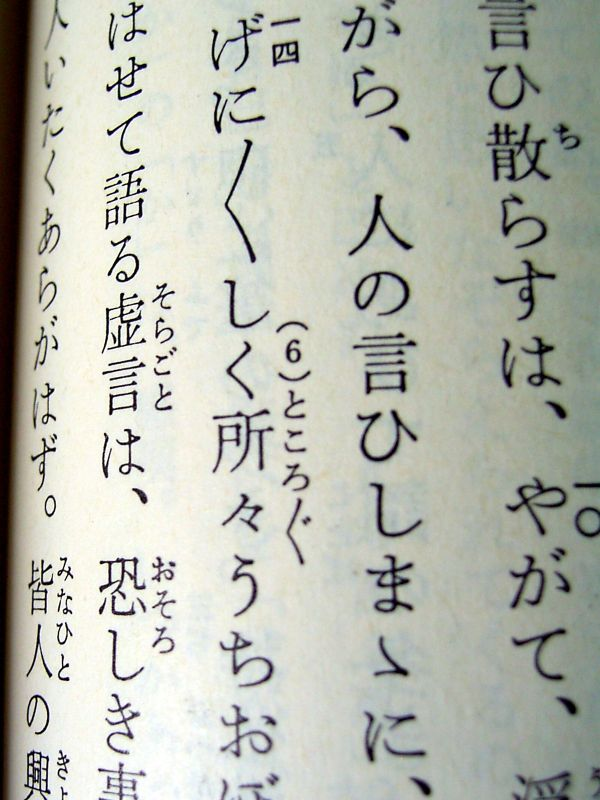
\includegraphics[width=0.35\textwidth]{tsuredzuregusa}
  \end{center}
  \caption{A sample of japanese text using iteration marks (long く; 々 ゝ).
  Japanese uses iteration marks extensively in its script.}
\end{wrapfigure}

In japanese writing there are 3 iteration marks. Given that japanese writes with
3 alphabets, these iteration marks correspond to the alphabet which is meant to
be iterated. For writing chinese characters (sinographs), 々 is used; ゝ for
hiragana; ヽ for katakana. If there are many of these symbols in a row, then
that many characters prior should be repeated. On top of this, if you want to
repeat a sound but change it slightly, such as changing \textit{ta} to
\textit{da}, then this can be shown by adding 2 dots to the iteration mark, as
japanese does to any character to show this type of change.

This would be impressive, but it is not all japanese has to offer. If writing
out these iteration characters more than once was too much, there are characters
for repeating several characters in a row: a single long く. This symbol is made
to a certain length, and how long it is shows how many characters to repeat.
This too can have dots added to show voicing of the first letter which is being
produced.

Moreover, japanese doesn't view iteration marks as improper. Although the use of
ヽ and ゝ has fallen in recent years, 々 is still considered part of the
standard spelling for hundreds of words. All of these marks are still frequently
used in historical texts and their reprints, and in stylized brand names such as
Isuzu (jp: «いすゞ».

\section{Objective}

We see that japanese makes powerful and systematic use of iteration marks
in formal and informal texts. For the latin script, a powerful technical
specification for marking repeated sections of text was developed in 1951
for use in \textit{regular expressions}. Regular expressions were originally
invented for the field of computer science, in which they are still widely used
today.

Regular expressions (RE) are sequences of characters which define a search
pattern. This will match with any text defined by the regular expression. As
part of its core specification, RE contains capabilities to match sequences
of any arbitrary characters, and specified repetitions of iteration of
characters. It is widely used in software development, and so is familiar to
software developers all over the world.

This paper describes an adaptation the syntax of core regular expressions to
common text to define a standard set of iteration marks. Moreover, we hope that
these iteration marks can be used beyond the original scope of the latin script
for the sake of transliterating iteration marks, which are used by languages as
diverse as arabic, khmer / lao / thai, japanese, chinese, indonesian / malay,
and egyptian hieroglyphs, sometimes as symbols not included in the standard
alphabet of that language.

\section{What is an iteration mark?}

\section{Context free iteration marks in regular expressions}

In RE, iteration is notated using braces (\{\}), an asterisk (*), or a plus sign
(+). Each of these symbols has a slightly different meaning. Normal brackets are
used to group text, and the absence of brackets indicates that only the
immediately preceding character is to be repeated.

Braces denote a fixed number of repetitions. For example, the RE «Hono(lu){2}»
matches with «Honolulu», and «e{3}k» matches with «eeek».

A period denotes any number of repetitions, including none. For example, the RE
«co*l» matches with «cl» and «coool» (or «cool» with any number of «o»s), and
the RE «(la)*» matches with any number of «la»s, such as «lalala» or
«lalalala», but doesn't match with «lalal».

Finally, a plus denotes any nonzero number of repetitions: The preceeding group
or character must occur at least once.

There is one final notation from RE which we find useful: saving and referencing
groups. This is done using brackets to select the group of characters, which can
then be referenced any time later on in the text using the positional
enumeration of that group (its position from the start of the text). This is
called \textit{positional referencing}.

Two examples of this are the REs «h(ocus) p(1)» (which matches with «hocus
pocus») and «(a)(b)(r(1))cada(2)(3)» (which matches with «abracadabra»).

Positional referencing works well for RE, but in practice is quite difficult for
people to read, especially in longer texts.

\section{Context free iteration marks}

We can adapt the notation of REs to indicate iteration in any text passages.
In order to make this easier to read and understand, the following changes are
introduced:

\begin{enumerate}
  \item Instead of using braces to indicate fixed iteration, we will instead
    use superscript.
  \item Instead of using brackets to indicate groups, we allow either brackets
    or underlines.
  \item Instead of using positional referencing to name groups, we let subscript
    letters or numbers name groups.
  \item When brackets are not used, the default is to repeat the entire previous
    word, including any space(s) that follow it.
\end{enumerate}

We see a few advantages in the first change. First, superscript iteration marks
are already popularized due to its use in mathematics to indicate
exponentiation. Second, this notation is also used in indonesian / malay and
filipino to indicate iteration. Third, this allows writers to choose between
easy input on a computer (where brackets are easier to use), or by hand
(where superscript is easier to use).

The second change also allows writers to choose between easy input on a
computer (brackets), or by hand (underline).

The third change makes referencing much easier for readers to follow. REs force
readers to count groups in order to figure out what group is being referenced
by a number. By allowing groups to be named to variables (or numbers),
referencing is made much easier for readers to follow.

The fourth and final change is a linguistic convenience. Reiteration is
incredibly common across all languages, and languages tend not to repeat
individual letters more than a few times in immediate succession; English rarely
does so more than 2 or 3 times in any word. It is therefore preferable to mark
repeated words (which take a long time to write) rather than letters (which are
commonly repeated but take almost no time to write).

Moreover, by allowing users to match with spaces that follow a word, we can
distinguish between common linguistic contrasts. For example, being able to
distinguish «blue \h{2} sky» («blue blue sky») from «blue\h{2} sky» («blueblue
sky»).

Finally, we add that all iteration in text should be case insensitive. Capital
letters are quite rare in text, and in most cases where iteration is used,
the copied text shouldn't match the case of the original text.

\section{Examples}

\subsection{English}

\begin{enumerate}
  \item blue \h{2} sky = blue blue sky
  \item blue\h{2} sky = blueblue sky
  \item Ki\h{2} = Kiki
  \item Bison \h{2} = Bison bison (A genus)
  \item Bye \h{2} = Bye bye
  \item Night \h{2} = Night night
  \item La\h{3} = Lalala
  \item Hono(lu)\h{2} = Honolulu
  \item B(aby)\s{a} shm\s{a} (shm-reiteration)
  \item \underline{Itsy}\s{x} b\s{x} spider = Itsy bitsy spider
  \item H\underline{ocus}\s{o} p\s{o} = Hocus pocus
\end{enumerate}

\subsection{Foreign language examples}

\subsubsection{Chinese}

\begin{enumerate}
  \item 人\h{2} = 人人 (or 人々 if using iteration marks)
  \item 蓝\h{2} = 蓝蓝 (or 蓝々 if using iteration marks)
  \item 乖\h{2} = 乖乖 (or 乖々 if using iteration marks)
\end{enumerate}

\subsubsection{Indo - european languages}

\begin{enumerate}
  \item Bon\h{2} = Bonbon (Various. en: «candy»)
  \item Taai\h{2} = Taaitaai (nl (dutch). en: «gingerbread»)
  \item Casi \h{2} = Casi casi (es-mx (mexican spanish). en: «almost»)
  \item Luego \h{2} = Luego luego (es-mx (mexican spanish). en: «later»)
\end{enumerate}

\subsubsection{Japanese}

Some of these examples make use of Japanese implicit voicing rules.

\begin{enumerate}
  \item (とき)\h{2} = ときどき
  \item (ところ)\h{2} = ところどころ
  \item 所\h{2} = 所々
  \item 日\h{2} = 日々
  \item い\h{3}んさつき = いいいんさつき (いい印刷機)
\end{enumerate}

Here we include an extract from «Yo ni kataritsutafuru koto» (JP:
«世に語り傳ふる事») to demonstrate how Japanese uses iteration marks in text.

\paragraph{Original}:

«げにゞゝしく所々うちおぼめき» % TODO: fix this with xelatex

\paragraph{Transliteration}:

«Geni\h{2} ni shiku tokoro\h{2} uchi obomeki» (Using implicit voicing)

\textbf{or:}

«Geni\h{2} ni shiku tokoro\s{x}d\s{x} uchi obomeki»


\label{sec:intro}
\end{document}

%%%%%%%%%%%%%%%%%%%%%%%%%%%%%%%%%%%%%%%%%%%%%%%%%%%%%%% End document contents %%

